Wir messen alle Abstände von $m_1$ aus: $m_1$ liegt bei $0$, $m_2$ bei $a$ und $m_3$ bei $a+b$. Im Schwerpunkt unterstützt, wäre der Stab im Gleichgewicht: Das Drehmoment der gesamten Gewichtskraft im Schwerpunkt ist gleich der Summe der einzelnen Drehmomente um $m_1$,
\begin{align}
 \left(m_1+m_2+m_3\right)g\cdot x_S &= m_1\,g\cdot 0 + m_2\,g\cdot a + m_3\,g\cdot\left(a+b\right)
\end{align}
Damit
\begin{align}
 x_S &= \xSpF \\
   &= \frac{\mSb\cdot\aSp+\mSc\cdot\left(\aSp+\bSp\right)}{\mSa+\mSb+\mSc} \\
   &= \xSp \approx \result{\xSpP{0}{2}}
\end{align}
Der Schwerpunkt liegt zwischen $m_2$ und $m_3$.

\begin{center}
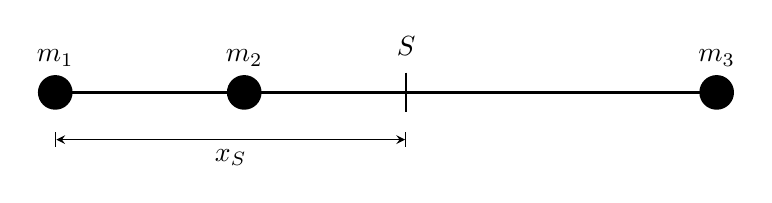
\begin{tikzpicture}[>=stealth]
 \draw[very thick] (0,0) -- (8.4,0);
 \fill (0,0) circle (0.22) node[above=6pt] {$m_1$};
 \fill (2.4,0) circle (0.22) node[above=6pt] {$m_2$};
 \fill (8.4,0) circle (0.22) node[above=6pt] {$m_3$};
 \draw[thick] (4.457,0.25) -- (4.457,-0.25);
 \node[above=4pt] at (4.457,0.2) {$S$};
 \draw[|<->|] (0,-0.6) -- (4.457,-0.6) node[midway, below] {$x_S$};
\end{tikzpicture}
\end{center}
